\documentclass{sig-alternate}
%[preprint]
% The following \documentclass options may be useful:
%
% 10pt          To set in 10-point type instead of 9-point.
% 11pt          To set in 11-point type instead of 9-point.
% authoryear    To obtain author/year citation style instead of numeric.

\makeatletter
\def\@copyrightspace{\relax}
\makeatother

\usepackage[nynorsk,british,UKenglish,USenglish,english,american]{babel}

\usepackage{graphicx}
\usepackage{tikz}
%\usepackage{gnuplot-lua-tikz}
\usepackage{color}
\usepackage{tabularx}
\usepackage{fixltx2e}
%% \usepackage{dblfloatfix}
\usepackage{varwidth} % http://ctan.org/pkg/varwidth
\usepackage{listings}
\usepackage{url}
\usepackage{balance}
\usepackage{amsmath}
\usepackage{enumitem}
\usepackage{caption}

\lstset{
%  backgroundcolor=\color{yellow!20},%
  basicstyle=\small\ttfamily,%
  numbers=left, numberstyle=\tiny%
}

\newtheorem{thm}{Problem}
\newdef{definition}{Definition}
\DeclareMathAlphabet{\mathpzc}{OT1}{pzc}{m}{it}
\newtheorem{theorem}{Theorem}[section]
\newtheorem{lemma}[theorem]{Lemma}

\usepackage{xcolor}
\usepackage{framed}
\usepackage{amssymb,amsmath}
\usepackage{ifxetex,ifluatex}
\usepackage{fancyvrb}
\usepackage{comment}

\begin{document}

\title{Pipelining an Open-Source Last-Level Cache}
% \subtitle{\large Kevin Yunchuan Jiang, Joseph Zuckerman\\
% \vspace{0.2cm} 
% \normalsize{\\
% kyj2112@columbia.edu\\
% Department of Computer Science\\
% Columbia University\\
% New York, New York, USA
% }
% }

\numberofauthors{3}
\author{
% \alignauthor
Kevin Yunchuan Jiang \qquad Joseph Zuckerman \qquad Luca P. Carloni \\
Department of Computer Science, Columbia University \\
kyj2112@columbia.edu, \{jzuck, luca\}@cs.columbia.edu 
}

\vspace{-2cm}

\maketitle

\vspace{-2cm}

% \begin{abstract}
% {
% Systems-on-chip (SoCs) have with increasingly complex integration primarily rely on on-chip shared memory for performance. Like caches on single-core processors,
% implementing cache-coherence via a cache hierarchy on a multi-core system can greatly improve performance and reduce energy consumption. Previous works have also shown that this can be
% extended to heterogeneous SoCs, which has the added complexity of managing accelerator memory accesses together with multi-core cache coherence.
% \par ESP is an open-source platform for hetergeneous SoC design that streamlines the integration of heterogeneous components in SoC architecture.
% The ESP architecture utilizes an extended MESI directory-based cache coherence protocol to implement cache coherence across the processors and accelerators in the system. The ESP cache hierarchy consists of L1/L2 caches that are coupled
% to the processors and accelerators, as well as a
% on heterogenous SoCs can also provide significant speedups and reduce off-chip memory accesses. One current limitation of 
% the ESP Last-Level Cache (LLC) is that it is implemented as a multi-cycle datapath that can only handle one request at a time. 
% This limits the throughput of the LLC in situations when multiple requests are issued in a short period of time.
% In order to increase the throughput of the LLC in such situations, we propose separating the 6 stages of the LLC datapath from its FSM controller
%  and implementing pipelining logic between each stage.
% Implementing pipelining in this fashion allows for handling multiple memory accesses and leads to better performance of multi-core SoCs.
% }
% \end{abstract}
\section{Introduction}
\label{sec:intro}

Systems-on-chip (SoCs) that integrate a heterogeneous mix of complex IP blocks
can utilize on-chip shared memory to improve performance and simplify
programming \cite{spandex, cohort, li2023duet, mantovani_cases16}.  Like that
of traditional homogeneous architectures, the memory hierarchy of heterogeneous
SoCs may feature multiple levels of caches, orchestrated by a cache coherence
protocol. For example, Giri et al. propose a cache hierarchy for heterogeneous
SoCs built on top of a network-on-chip (NoC) \cite{giri18}.  Their cache
hierarchy supports multicore execution of processor cores and enables multiple
different coherence modes for hardware accelerators.  Utilization of these
modes can improve execution time and reduce off-chip memory accesses for a
variety of different workloads \cite{giri_ieeemicro18, zuckerman_micro21}.

\par ESP is an open-source platform for heterogeneous SoC design that simplifies
the integration of new IP blocks within a scalable SoC architecture and allows
for rapid prototyping of full systems \cite{mantovani_iccad20}. ESP's cache
hierarchy implements the protocol proposed by Giri et al -- an extended MESI
directory-based protocol.  The L1 of open-source processors (that potentially
implement different ISAs) interfaces to the ESP L2. The last-level cache (LLC)
and directory controller not only orchestrate coherence across these L2 caches
but also enable accelerators without a private cache to leverage the cache
hierarchy to access on-chip shared data.

\par In this work, we present an improved version of the ESP LLC. While the
original version is implemented with a multi-cycle datapath, the improved
version features a pipelined datapath, allowing for significantly greater
throughput. Since the last-level cache is the main synchronization point for
the various IPs throughout an SoC, this can give significant performance
improvements when there is a high density of requests at the LLC. In
particular, we show how the pipelined datapath can improve the performance of
accelerators that access their data directly from the LLC.

\section{The ESP Cache Hierarchy}
\label{sec:cache}

Figure \ref{fig:esp_tile} shows an example of a 4x4 tile ESP system with
elements of the memory hierarchy highlighted; the heterogeneous mix of tiles are
connected by a multi-plane network-on-chip (NoC).

ESP's coherence protocol is implemented by the L2 and last-level caches.  Each
\emph{Processor Tile} contains an open-source core, instantiated off-the-shelf
with its own L1 cache. The ESP L2 allows different cores to seamlessly
participate in ESP's coherence protocol, despite having potentially different
ISAs, endianness, and interfaces.  \emph{Accelerator Tiles}, which instantiate
a \emph{loosely-coupled accelerator}, can also optionally be equipped with
their own private L2 cache, which allows them to also participate in the
coherence protocol, just like processor cores.

The \emph{Memory Tile} contains the LLC and directory controller, which manage
coherence among all L2 caches in the system, and a channel to external DRAM.
The LLC can be partitioned across multiple memory tiles in the system with each
partition serving a discrete partition of the global address space and
providing its own channel to DRAM. The LLC can also handle DMA requests
directly from accelerators, saving off-chip memory accesses in many
circumstances.

\par Compared to the L1 and L2 caches, the LLC contains additional metadata for
all cache lines active in the system at any point, such as which cores own or
share the cache line. These metadata are necessary for the execution of the
extended MESI directory-based cache coherence protocol.  In addition to the
standard MESI states (Modified, Exclusive, Shared, Invalid), the ESP coherence
protocol introduces a Valid state, which corresponds to lines that are not
owned or shared by any private cache. Maintaining a Valid state saves an
off-chip memory access to subsequent requests for this line; it is also used to
represent lines that have been accessed by an accelerator through DMA to the
LLC. Valid lines are also the first choices for evictions.

The various caches and processing elements in ESP communicate through the NoC.
Three NoC planes are used for coherence requests, responses, and forwards,
while two planes are used for DMA requests and responses from/to accelerators.

%\begin{figure}[h]
%  \centering
%  \captionsetup{justification=centering, format=hang}
%  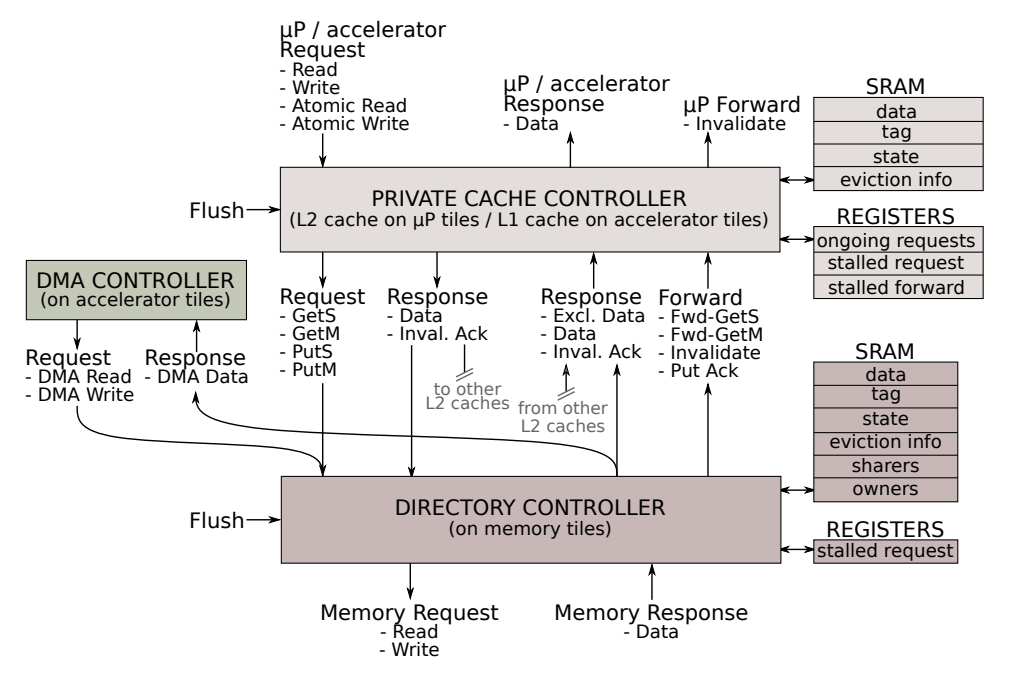
\includegraphics[width=1\columnwidth]{fig/esp_hier.png}
%  \caption{ESP Cache Hierarchy~\cite{giri18}}
%  \label{fig:esp_hier}
%  \end{figure}

\begin{figure}[t]
  \centering
  \captionsetup{justification=centering, format=hang}
  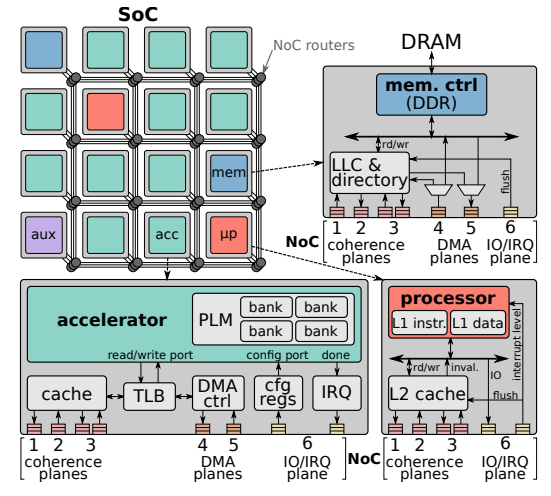
\includegraphics[width=1\columnwidth]{fig/noccache.png}
  \caption{Detailed ESP Tile Grid~\cite{giri18}}
  \label{fig:esp_tile}
  \end{figure}


\pagebreak
\section{Pipelining the ESP LLC}
\label{sec:llcImplementations}
\subsection{Original LLC}
The original LLC is implemented as a multi-cycle datapath for handling requests
according to the extended MESI protocol. The multi-cycle datapath consists of
six stages, and an FSM manages the execution of a single request across these
six stages.  In any given cycle, only one stage of the datapath is active. For
example, the first stage, which prioritizes and accepts the incoming requests,
is idle while later stages of the datapath are operating. This means that only
one request is processed by the LLC at a time, which can create backpressure
on the NoC if many requests arrive in a short time.
\subsection{Pipelined LLC}
In this work, we took the existing six-stage datapath and enabled the pipelined
execution of requests. We use the same six stages from the multicycle datapath
and add pipeline registers in between each stage and logic for exerting backpressure
between individual stages. The FSM that governs the execution of an individual request
is removed, all stages can be active in any given cycle. This implementation allows
for the simultaneous processing of multiple requests.

\par Pipelining a multi-cycle datapath presents numerous challenges. Signals
from previous stages that would previously stay constant throughout the
lifetime of a request now can be overwritten by new requests. This required
significant refactoring of the RTL to pass these signals with each request
through the pipeline.

\par The cache itself is a multi-bank, multi-port memory that allows for an
entire set to be read in a single clock cycle. This applies to the cache lines
themselves and also their associated metadata. Another key challenge is
avoiding read-after-write (RAW) hazards and read/write collisions within a
particular set.  RAW hazards can occur because the memory is not updated until
the final pipeline stage, while it is read in the second stage. Without careful
consideration, it would be possible for a new request to read information about
a set before an old request updates the data. It is also necessary to avoid
reading and writing the same location in this memory during the same clock
cycle to avoid non-determinism in accesses. To solve these two hazards, we introduce
a \emph{set table}, which keeps track of the sets of all requests currently active
in the pipeline. The second stage of the pipeline checks the set table before accepting
new requests in order to avoid multiple requests to the same set in flight at once. The final
pipeline stage removes an entry from the set table when it is retired. Requests
in different sets do not face these hazards, but they pose a different problem:
the memory architecture of the original LLC was not designed for simultaneous
reading and writing; we expanded the number of ports in the memory to sustain
higher throughput.

\par Pipelining the multi-cycle datapath also introduced potential for
undesired out-of-order completion of requests. There are two problematic cases:
when the LLC wants to recall an Exclusive or Modified cache line from an L2 for
eviction and when there is a cache line in a transient state waiting for a data
response from an L2. In both cases, the LLC should not service any newer
requests until the data response from the L2 has been received and completely
serviced. However, these behaviors are only determined at the fifth stage of
the pipeline, and so new requests can enter the pipeline before the response is
received.

Our solution was to add a feature to the fifth stage that stalls the first
stage and flushes all the newer requests in the pipeline into a FIFO. After the
data response has been received and serviced, the LLC will process the requests
in the FIFO before accepting any new requests from externally.
LLC will then prioritize feeding requests from the FIFO back into the pipeline
once the data response has been received and serviced.

\par While the original LLC significantly improved DMA latency for accelerators
by potentially eliminating off-chip memory accesses, the pipelined LLC
further improves DMA performance. Large DMA requests span multiple
cache lines, and the LLC handles each cache line as a separate
"request" for a different address. The pipelined LLC is designed to generate a
new "request" to insert into the second pipeline stage every cycle, allowing
the DMA request to fully utilize all stages of the pipeline. When the accelerator
data resides in the LLC, this allows a new cache line to be sent or written every
cycle, as opposed to every six cycles in the old implementation.

\section{Performance Test Results}
\label{sec:performanceTestResults}
To compare the performance of the two implementations, 
we synthesized each implementation as part of a SoC, programmed the SoCs 
onto the same FPGA boards, and ran 3 types of accelerator applications on the FPGAs. 
Both SoCs have three different accelerators for the three applications: 
Fast Fourier Transform (FFT), General MAtrix Multiply (GEMM), and 2D convolution (CONV2D). 
For each application, we used 5 workload sizes from extra small (XS) to extra large (XL). 
We also tested each application under 2 different coherence modes: LLC-Coherent (Accelerators 
have no L2 cache and only interface with the LLC for coherence) and Coherent (Accelerators 
have L2 caches that are coherent with other L2 caches in processors). While running the applications, 
we measure the number of cycles that the accelerator spends communicating with memory.

\par Figure \ref{fig:dma_chart} shows the speedups calculated from the results of our testing. 
While the speedup for CONV2D stays relatively constant across different workloads, 
the speedup is much larger for FFT and GEMM at smaller to medium workloads. This is 
to be expected, as these workload sizes will allow the accelerators to benefit the most from the improved 
DMA execution of the pipelined LLC. For larger workloads, the accelerators will be primarily receiving 
un-cached data from main memory, so the speedup is not as significant. 


\begin{figure*}[t]
    \centering
    \captionsetup{justification=centering, format=hang}
    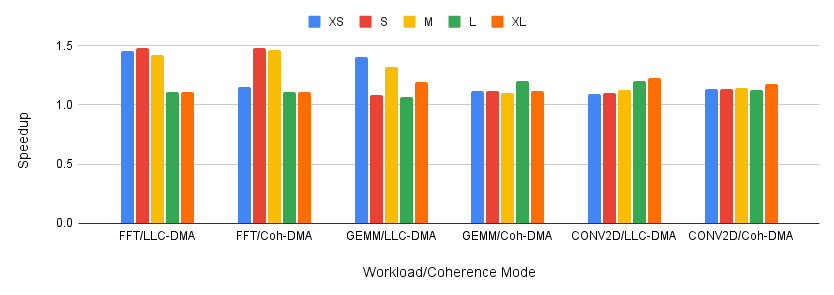
\includegraphics[width=1\textwidth]{fig/DMA_chart.png}
    \caption{Speedup of Pipeline LLC compared to Original LLC for various sizes of applications under different coherence modes. LLC-DMA refers to LLC-Coherent, and Coh-DMA refers to Coherent.}
    \label{fig:dma_chart}
    \end{figure*}
  

% \begin{figure}[h]
%   \centering
%   \captionsetup{justification=centering, format=hang}
%   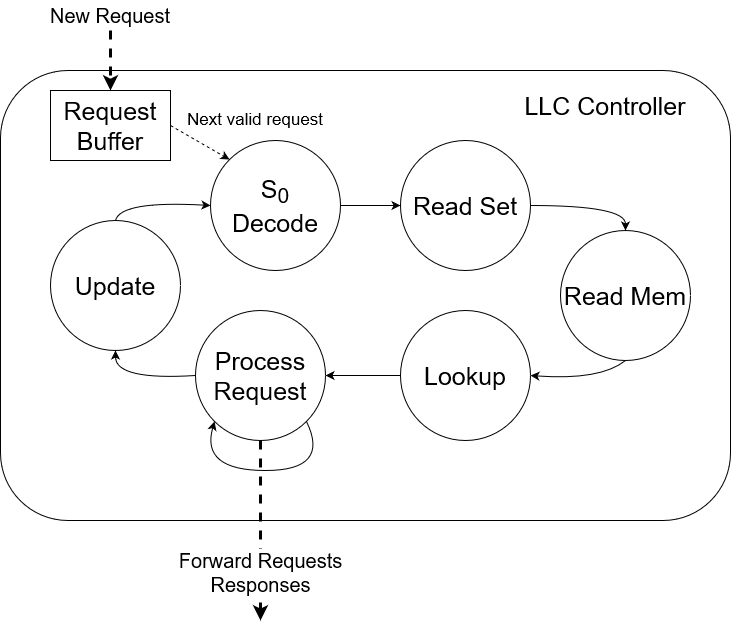
\includegraphics[width=1\columnwidth]{fig/LLC_Core_FSM_fa22.png}
%   \caption{LLC State Machine}
%   \label{fig:llc_fsm}
%   \end{figure}

% \subsection{Unpipelined Implementation of LLC} %%Kevin
% The unpipelined implementation of the LLC utilizes state machine controller to move between 6 states of handling a request. Each request is handled according to the MESI Directory Protocol.
%  The LLC controller is shown in Figure~\ref{fig:llc_fsm}. Each state, with the exception of Process Request takes one cycle. Process Request may take one or more cycles, depending on the type of request.


% \par In the actual RTL code, the LLC consists of several SystemVerilog modules. The modules are shown in detail in Figure~\ref{fig:llc}.
%   The LLC Core module contains the LLC Controller, which is responsible for activating enable signals to the Input Decoder, Address Decoder, Buffers, Lookup, Process Request, and Update modules.
%   These six modules form the multi-cycle datapath for processing requests.
%   Each of these modules correspond to one of the states in the state machine shown in Figure~\ref{fig:llc_fsm}.
%  The LLC Controller initially starts in Decode state. Requests from outside the LLC can only be accepted in this state. Requests 
%  that come into the LLC while the LLC controller is not in this state will cause the request to be stored in the Request Buffer.
% \begin{itemize}
%   \item In the Decode state, the Input Decoder module is enabled by the LLC controller. During this stage, the LLC controller takes in a request from
%   outside the LLC. At the end of this clock cycle, the Input Decoder outputs control signals according to request type.
%   \item In the next clock cycle, the LLC controller moves into the Read Set state and enables the
%   the Address Decoder module. The Address Decoder combinationally decodes the cache set and tag from the address specified in the request.
%    During this state, the decoded cache set is also combinationally sent to the Local Memory module. At the end of the cycle, the Local Memory will output the data stored in the cache lines of the cache set.
%   \item In the next clock cycle, in the
%   Read Mem state, the Buffers module is enabled, and the requested data from Local Memory is stored into the Buffers.
%   \item In the next clock cycle, in the Lookup state, the Lookup 
%   module is enabled. In this state, the data inside the Buffers is checked for a tag hit/miss.
%   \item The next state, Process Request, may take multiple cycles. In this state, the LLC controller enables the Process Request module, which outputs the correct data responses, forward-requests,
%   or memory requests according to the control signals. In certain cases, such as when a processing unit requests a piece of data that is currently
%   in the Invalid state, the Process Request module must send out a request to Memory and wait for a response, which will last several cycles. The Process Request module may also write new data into the Buffers module.
%   \item The Update state takes any new data written to the Buffers during Process Request and writes it to Local Memory.
%   \item Finally, the LLC controller returns to the Decode state and starts to takes in the next request.
% \end{itemize}
% In this implementation, only one module in the multi-cycle data path is enabled in any given clock cycle. The Input Decoder, Memory Buffer, and Lookup modules are all idle during the Process Request state. The LLC controller maintains
% a Request Buffer of size 1, but any more requests will result in backpressure signals from the LLC. This is inefficient because
% the Process Request state may last several clock cycles, and other processing units cannot
% issue any new memory requests during this time. Instead of keeping the earlier modules
% in an idle state, the next few requests can start being decoded, and cache hits/misses can start being checked. To achieve this, we attempt to decouple the earlier modules from the LLC Controller, 
% implement pipeline buffers in between these modules, and add pipelining logic.
% \par It is important to note that the outputs of each module in the multi-cycle data path are not only connected to the next module in the data path. For example, the output control signals from the Input Decoder 
% module is recieved as inputs by the Address Decoder module, the Process Request module, and the Update module. This is not a problem in this implementation because the LLC controller de-enables the Input Decoder 
% module and prevents its output form changing for the entire multi-cycle data path. However, as will be discussed in the following section, these kinds of signals are the main challenge in pipelining this cache design.

% \begin{figure*}[h]
%   \centering
%   \captionsetup{justification=centering, format=hang}
%   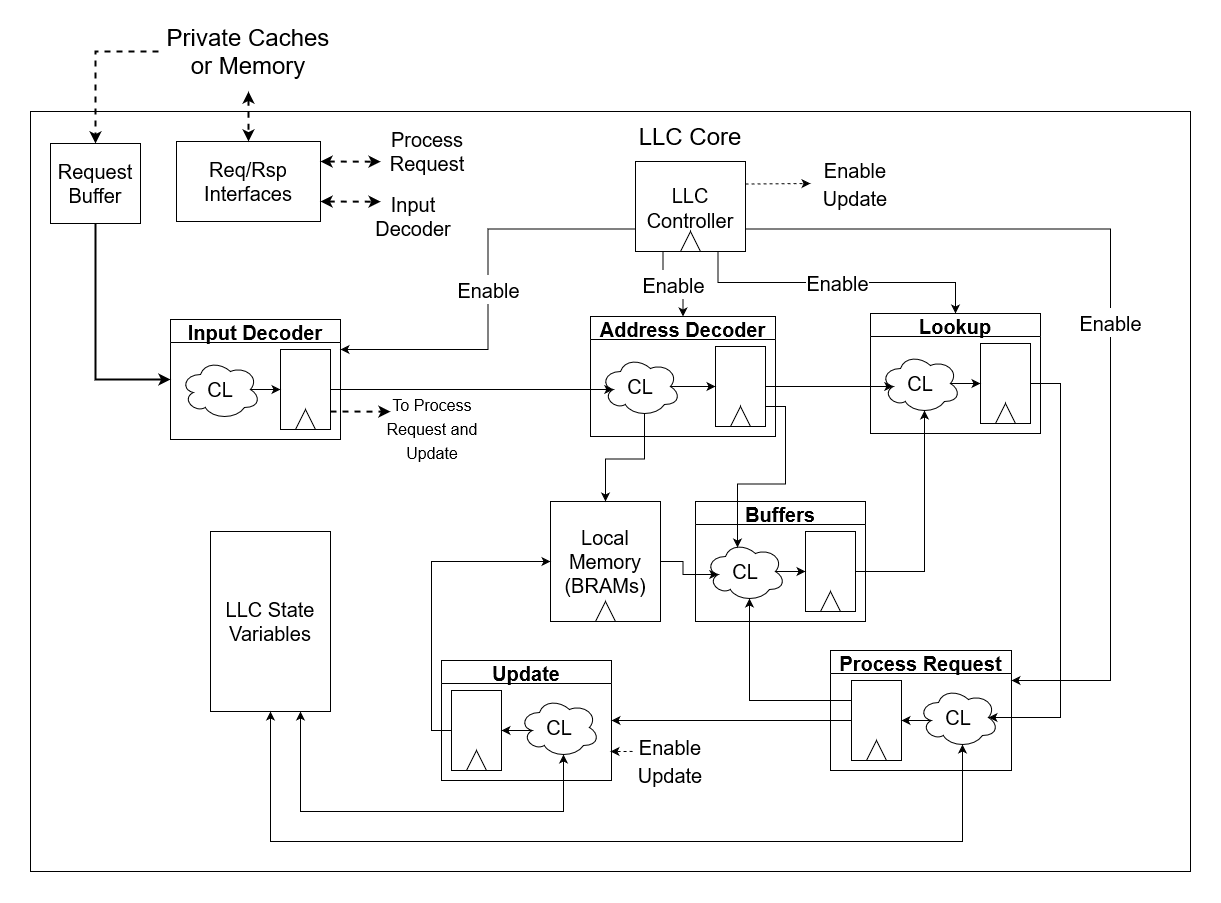
\includegraphics[width=1\textwidth]{fig/LLC_RTL_Unpipelined_3.png}
%   \caption{Unpipelined LLC RTL Modules}
%   \label{fig:llc}
%   \end{figure*}

% \begin{figure*}[h]
%   \centering
%   \captionsetup{justification=centering, format=hang}
%   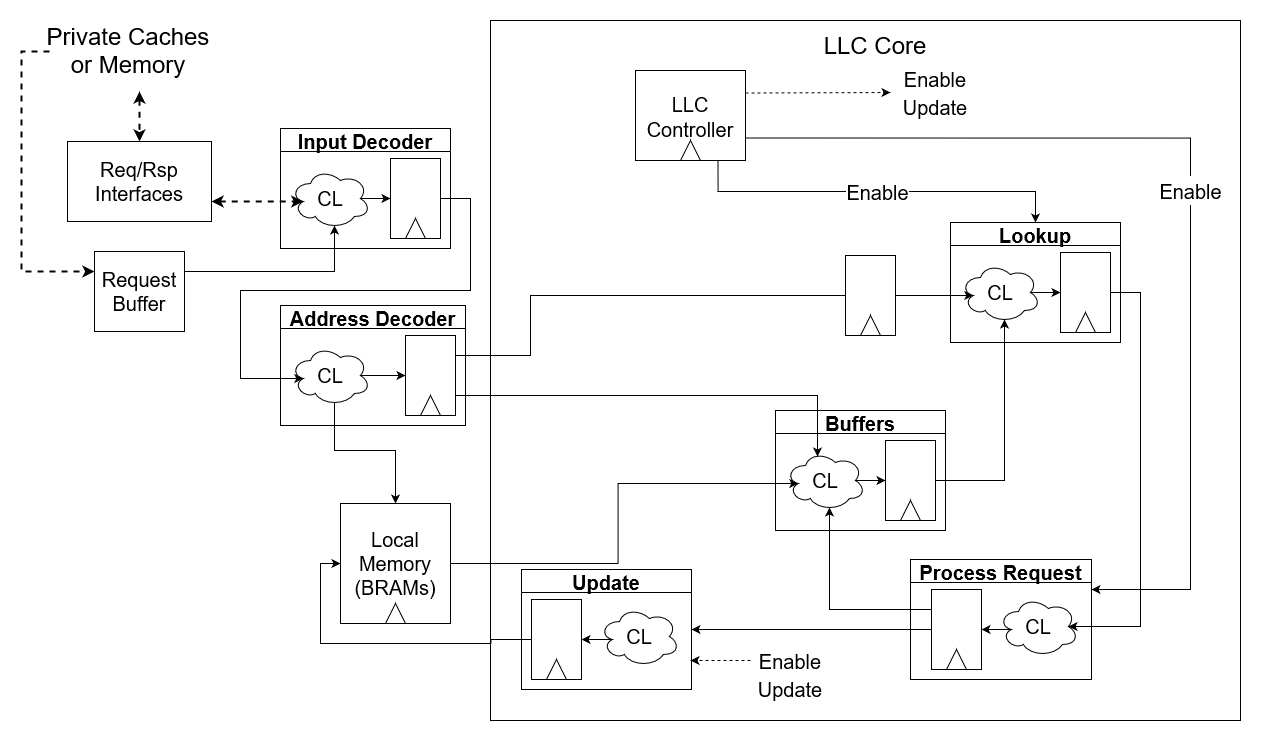
\includegraphics[width=1\textwidth]{fig/LLC_RTL_Pipelined_4.png}
%   \caption{Pipelined LLC Block Diagram}
%   \label{fig:llc_pipelined}
%   \end{figure*}

% \subsection{Pipelined Implementation of LLC} %%Kevin
% The most recent implementation of the Pipelined LLC is shown in Figure~\ref{fig:llc_pipelined}. This implementation builds open what we had accomplished in the Spring 2022 Semester. During the Spring 2022 semester, 
% four major accomplishments were made:
% \begin{itemize}
%   \item Pipeline buffers using FIFOs were inserted between each module. We chose to use FIFOs as our pipeline buffers because
%   FIFOs have built-in valid and ready signals (full, empty, push, pop) that can be used for back pressure and other pipelining logic within the 
%   modules. Additionally, our implementation of the FIFO can take in custom data types. Custom data types are important because there are a large number 
%   of different signals going between each module, and every signal needs to be pipelined. Rather than allocating a register for each individual signal, 
%   we chose to pack the signals into custom data types to be passed into the FIFO.
%   \item Custom data types were created for each set of signals between modules. We used SystemVerilog packed structs to combine multiple signals into a single data type. In total, 
%   we implemented five custom data types for each pipeline FIFO. Each FIFO handles different sets of signals, so five different data types were necessary. Additionally, 
%   we implemented logic for flattening 2D bit arrays into 1D bit arrays. SystemVerilog packed structs only accept 1D bit arrays as part of its constituent data, but some signals inside the LLC 
%   are implemented as 2D arrays. In order to pipeline these signals through the FIFO, they must be flatted and un-flatted at the input and output of the FIFO.
%   \item The Input Decoder module was decoupled from the FSM controller. Instead of using an enable signal from the LLC Controller, the Input Decoder is now always active and communicates directly with the rest of the cache
%    hierarchy. Upon receiving a new request from the outside, the Input Decoder will push the result control signals into the FIFO buffer between the Input Decoder and the Address Decoder. When the FIFO buffer is full,
%    the Input Decoder will send backpressure to the outside. When the FIFO buffer is empty, the Input decoder will tell the outside that the LLC is reeady for a new request.
%   \item In order to preserve the correctness of the LLC after pipelining, we re-routed important signals from the Input Decoder. As shown in Figure~\ref{fig:llc}, the original implementation 
%   routes control signals directly from the Input Decoder directly to the Process Request and Update modules. This works when the FSM controller is in control of all modules, because 
%   the Input Decoder will not be active during later stages, and the control signals will stay the same. However, after decoupling the Input Decoder from the FSM controller, the Input Decoder can now handle a second request after 
%   a first request enters the FSM controller. When the Input Decoder handles the second request, the output control signals will change, and the Process Request module will now have the control signals corresponding to the second request instead of the first request.
%   To solve this issue, we routed the control signals of the Input Decoder through FIFO buffers between each module, as shown Figure~\ref{fig:llc_pipelined}. The control signals enter the FSM controller together with the request data. At each state, the control signals propagate through one pipeline FIFO. 
%   When the control signals reach the FIFO before the Process Request module, they stay there until the Process Requests completes its task and sends a pop signal to the FIFO. This ensures that the correct Correct Signals will be inputted into the Process Request sub-module for the entirety of the Process Request state. 
% \end{itemize}
% \par Our work in the Spring 2022 semester still left many bugs to be solved. The unpipelined implementation of the LLC came with a testbench to verify the funtionality of the RTL code. The implementation at the end
%  of the Spring 2022 semester was unable to pass the unpipelined testbench. There would also be incorrect responses when this implementation received two consecutive requests.
% \par This semester, three major accomplishments were made:
% \begin{itemize}
%   \item We fixed the Spring 2022 implementation so that it could fully pass the unpipelined LLC testbench. This verifies the functional correctness of our code when used in contexts that do not require pipelining,
%    and was an important first step. To acheive this, we needed to remove some LLC state variables and send them through the pipeline instead. The LLC State Variables module can be seen in Figure~\ref{fig:llc}. These
%    state variables output to multiple modules within the datapath, and they are meant to stay constant during the multi-cycle datapath, similar to the control signals from the Input Decoder. However, multiple modules
%    also modify these sate variables when they are active. The Input Decoder, now decoupled, would modify these state variables at the wrong time. While we did not completely remove the LLC State Variables module,
%    we removed the module from Figure~\ref{fig:llc_pipelined} to show the changes that we made. 
%   \item We decoupled the Address Decoder and Local Memory modules from the LLC Controller and passed the unpipelined LLC testbench. There were many challenges when achieving this. First, the cache set that is decoded
%    by the Address Decoder needed to be pipelined so that the Update Module could use it a few cycles later. However, the cache set also needed to be sent combinationally to the Local Memory module in the current cycle.
%    As as result, we needed to implement additional logic inside the Local Memory module to choose the right set (from Address Decoder or from Update). We also found out that the Process Request module was using data
%    directly from the Req/Rsp Interfaces module, as shown in Figure~\ref{fig:llc}. This module contains all the data for the current request coming into the LLC, such as the memory address being requested. However, since
%    the current request coming in is different from the request already in the pipeline, the Process Request would end up using the wrong address. To solve this, we needed to create a new data structure to store all
%    the fields of the request, because the Req/Rsp Interfaces module uses the SystemVerilog interface construct, which cannot be part of a SystemVerilog packed struct. This data structure is then used to send the request fields
%    through the pipeline so that the Process Request module will have the correct request fields a few cycles later.
%   \item We set up a pipelined LLC testbench which sends three consecutive requests into the LLC. The most recent LLC implementation is able to receive all three requests and send out the correct responses.
% \end{itemize}

% \section{Evaluation}

% \subsection{Unpipelined LLC testbench}
% As described in the previous section, the unpipelined LLC testbench is used as the first test for the LLC. Whenever we decouple a module, we need to first pass this testbench. The current implementation with both
%  the Input Decoder and Address Decoder decoupled is able to pass this testbench.

% \subsection{Pipelined LLC testbench}
% This testbench is a modified version of the unpipelined LLC testbench. Instead of sending one request and waiting for one response at a time, this testbench sends in three consecutive requests and waits for
%  three consecutive responses. Currently, this testbench is extremely short and only tests one type of request at a time. However, the fact that our LLC implementation is able to pass this testbench means that
%  the pipeline capability of the LLC is now functionally correct. The results of this testbench versus the results of a shortened unpipelined testbench can be seen in Figure~\ref{fig:mult_puts} and Figure~\ref{fig:puts}. The pipelined testbench ended
%  three cycles earlier thanks to the pipelining.

% \subsection{ESP Full System simulation}
% The current LLC implementation was also tested in the ESP full system simulation, because it had already passed the unpipelined testbench. However, the current implementation only passes a portion of the simulation,
%  and debugging is still in the process.

%  \begin{figure*}[h]
%   \centering
%   \captionsetup{justification=centering, format=hang}
%   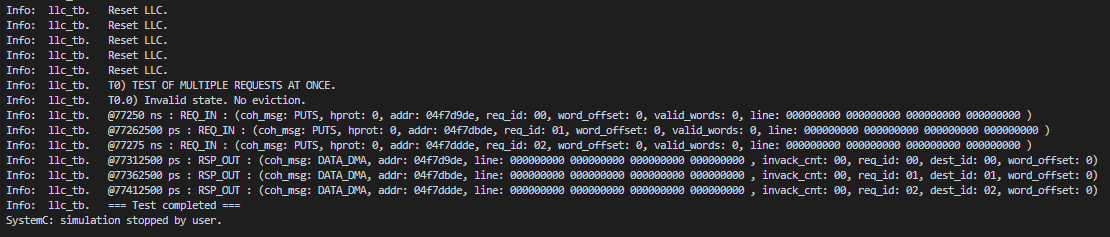
\includegraphics[width=1\textwidth]{fig/mult_puts_success.PNG}
%   \caption{Pipelined Testbench Results}
%   \label{fig:mult_puts}
%   \end{figure*}

% \begin{figure*}[h]
%   \centering
%   \captionsetup{justification=centering, format=hang}
%   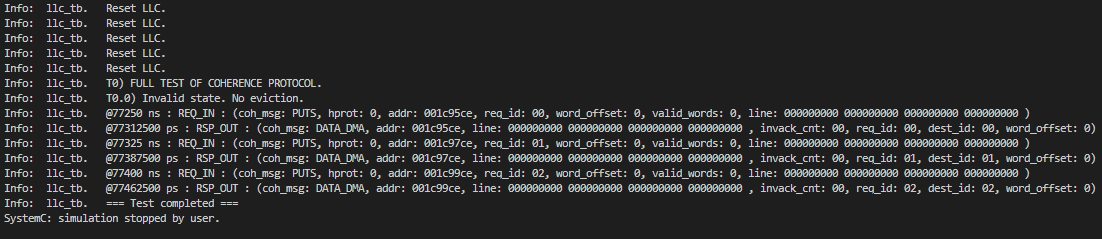
\includegraphics[width=1\textwidth]{fig/puts_success.PNG}
%   \caption{Unpipelined Testbench Results}
%   \label{fig:puts}
%   \end{figure*}



% \section{Future Work}
%  \begin{itemize}
%    \item The remaining stages have yet to be decoupled. The Buffer module is the next module in the data path. Since it is used for both writing and reading to and from Local Memory, there will be additional challenges
%    to implementing it.
%    \item The current LLC does not yet pass the ESP full system simulation. Even without fully decoupling the stages, work can still be done in parallel to debug the LLC so that it passes the simulation. 
%    This would also be more productive in fully verifying the functoinality of the LLC. Once the LLC passes the simulation, we can get to FPGA testing.
%    \item The pipelined LLC testbench needs more work so that it can test more types of requests for a longer period of time.
%  \end{itemize}

%Bibliography
{\small
%\bibliographystyle{abbrv}
\bibliographystyle{unsrt}
\bibliography{ref}
}


% If you need to add an appendix with large figures or table use the following
% code:

%% \newpage
%% \onecolumn{
%% \centering
%% \section*{APPENDIX}
%% \vspace{0.5in}

%% % Add your Appendix text and figures here.

%% }

\end{document}
